\documentclass{article}
\usepackage[preprint,nonatbib]{neurips_2024}
\usepackage{amsmath}
\usepackage{graphicx}
\usepackage{fontspec}
\usepackage{url}
\usepackage{tikz}
\usepackage{float}
\usepackage{siunitx}
\setmainfont{Times New Roman}

\title{Aurora Echo -- Audio-visual Service Feedback System}
\author{
    Ethan Goh \\ \texttt{7086cmd@gmail.com} \\ Zhenhai High School
        \thanks{The article is written during the summer camp held by Shanghai Jiao Tong University, which provides us a stage to crate innoative applications with artificial intelligence. Ethan Goh's Chinese Pinyin name: Wu Chengyu. Ethan Goh designed the project and the architecture of the system, and takes the responsibility of the development.}
    \and Bingzhen Wu \\ Zhenhai High School \thanks{Wu develops some extensions for the system, and takes the responsibility of the testing.}
    \and Qinyu Wang \\ Zhenhai High School \thanks{Wang makes the presentation for the project, and participate in the development.}
    \and Pengzhi Chu \\ Shanghai Jiao Tong University
    \and Xiaoni Liang \\ Shanghai Jiao Tong University
}
\date{\today}

% Document
\begin{document}
    \maketitle

    \begin{abstract}
        Service feedback systems are widely used in daily life, but the traditional text feedback system is not vivid and direct enough.
        Users will only give its rate and sometimes write a few words, or be required to fill in a blank with staggering amount of questions, which is not enough for the resource provider to improve its service.
        In this paper, we propose a new feedback system, named \textbf{Aurora Echo}, which provides audio-visual feedback for the resource provider.
        Through numerous artificial intelligence, such as LLM, we can make the system more friendly to not only user but also the resource provider.
    \end{abstract}

    \newpage

    \section{Introduction}\label{sec:intro}

    In daily life, resource provider may want users to provide the feedback of the resource\cite{åström2010feedback}, but in text form, it is hard to capture the direct response, including the facial emotion, the sense of speaking.
    In text form, we sometimes rate it as 5 stars, but in fact we are not satisfied with the service, since we just want to get the reward, or we are too lazy to write the feedback.
    It is also boring to type comments, especially facing the ``50 words at least'' and similar requirement.

    Is there a way to provide feedback in a more vivid and direct way?
    Associating the video conference, we adapted the form and integrate artificial intelligence algorithms to provide a more vivid and direct feedback system.

    The \textbf{Aurora Echo} system, as we named, is a system that provides audio-visual feedback for the resource provider.
    It mainly uses \texttt{transformers}\cite{DBLP:journals/corr/abs-1910-03771} provided by HuggingFace, \texttt{PyTorch}\cite{DBLP:journals/corr/abs-1912-01703} provided by Meta, and \texttt{MediaPipe}\cite{DBLP:journals/corr/abs-1906-08172} provided by Google, to recognize the facial emotion, the sense of speaking, and the content of the speech.
    Then we can use Large Language Models (LLMs), such as Llama-3, to summarize and analyze the feedback, giving effective response to the resource provider and the feedback giver.

    The innovative parts of the project are:

    \begin{itemize}
        \item The system uses the audio-visual way (inspired by video conference) to fetch the feedback, which is more vivid and direct.
        \item The system introduces Large Language Models (LLMs) to summarize and analyze the feedback.
        We can use LLMs to generate the response to the IS-friendly format, to statistic the feedback, and help the resource provider to improve its service.
        \item Privacy is considered in the system.
        We apply mosaic to the video feedback, and we do not store the video feedback, only the audio feedback and the analysis.
        \item The interface for frontend.
        We provide a web interface for not only the resource provider to check the feedback and the analysis, but also the feedback giver to feedback the response and track the feedback.
    \end{itemize}

    \section{Background}\label{sec:back}

    The traditional feedback system experienced a long history.
    From the users, the feedback is the most direct way for resource providers to know how the users feel about the resource.\cite{hogan2007}

    First, people use suggestion boxes to collect feedback.
    It can be regarded as the first step of the feedback system.
    Users are required to write down their feedback on a piece of paper and put it into the suggestion box, which takes a long time to collect and analyze the feedback.

    Then, companies may contact customers to have a survey or an interview.
    It makes the process of feedback more direct, but it still requires a lot of time and human resources.
    With the proliferation of cell phones, companies may employ the SMS or email to collect feedback, which is more efficient than the traditional way.

    Nowadays, companies may ask users to rate the service in several seconds, or provide a form to fill in.
    It is friendlier to the automation system, but either user's time or the completeness of the feedback is not enough.

    Above all, the traditional feedback system requires a lot of human resources, and the feedback is not vivid and direct enough.
    With the development of LLMs, people may use Large Language Model to analyze the text feedback, but still, the most immediate aspect cannot be represented.

    \section{Architecture}\label{sec:arch}

    The figure~\ref{fig:basic-arch} shows the basic architecture of the \textbf{Aurora Echo} system.
    The \textbf{Aurora Echo} system is mainly composed of three parts: the audio process system, the visual recognition system, and the feedback analysis system.
    Beside of the core system, we also provide a web interface for the resource provider to check the feedback and the analysis.

    \begin{figure}[hhhh]
        \centering
        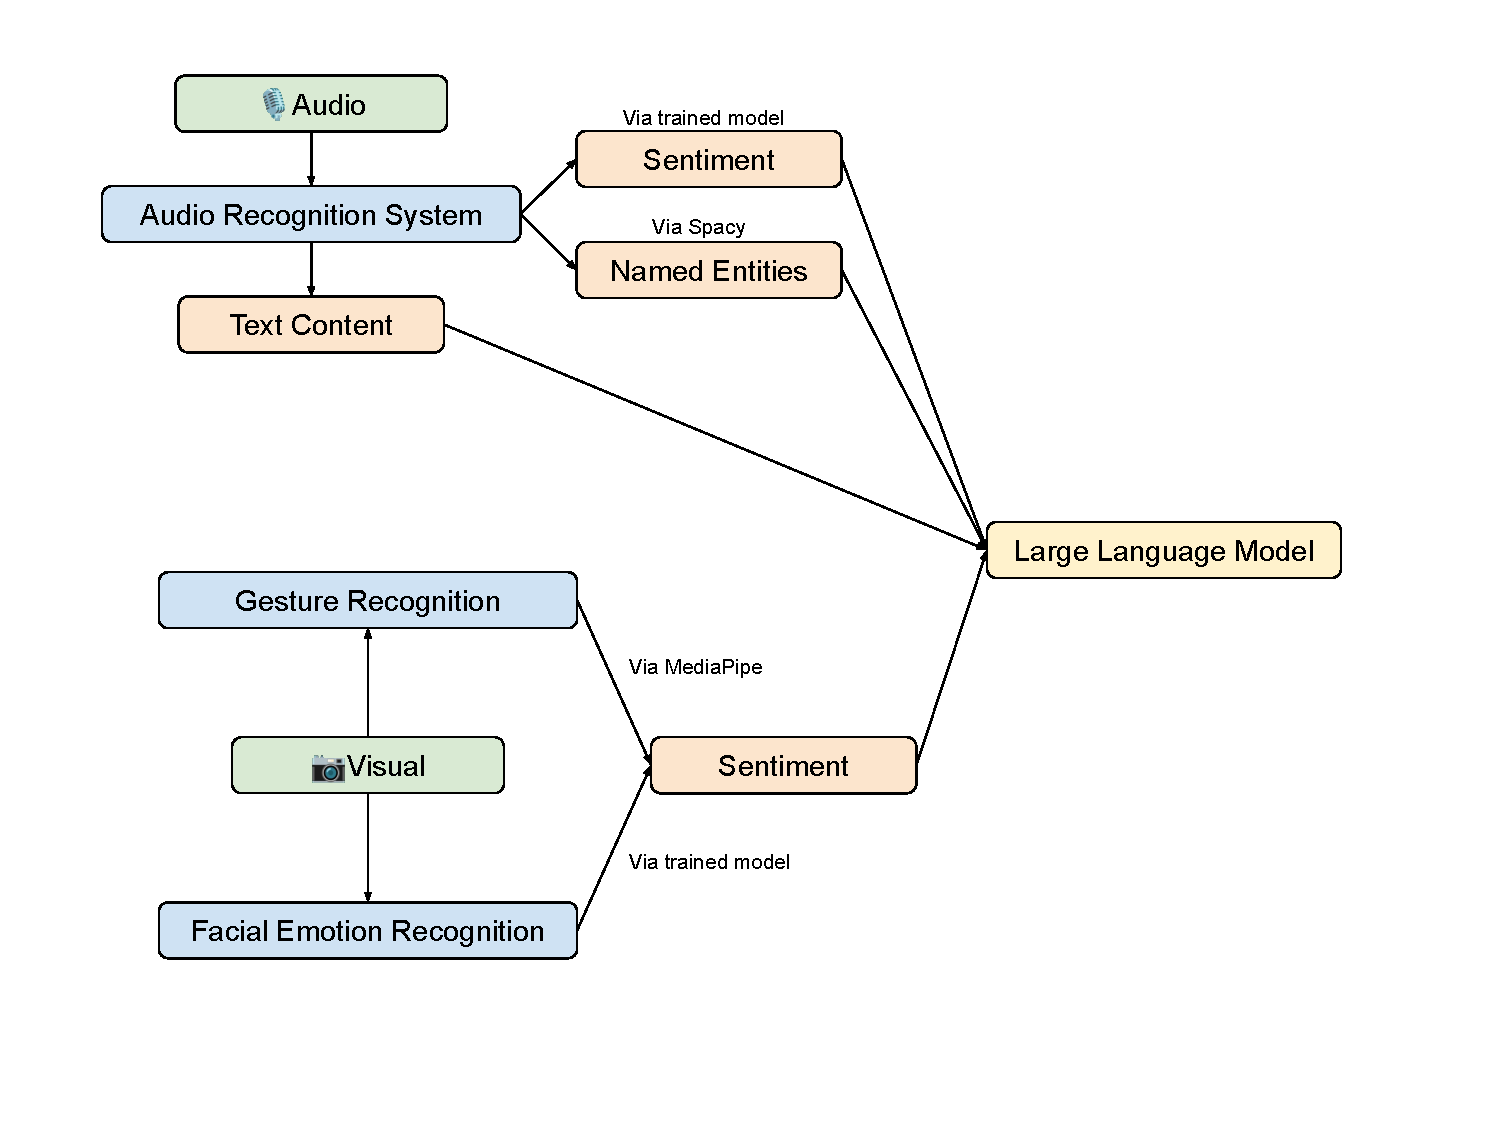
\includegraphics[width=0.8\textwidth]{./figures/basic-arch}
        \caption{The basic architecture of the \textbf{Aurora Echo} system.}
        \label{fig:basic-arch}
    \end{figure}

    \subsection{Audio Process System}\label{subsec:audio}

    \begin{figure}[hhhh]
        \centering
        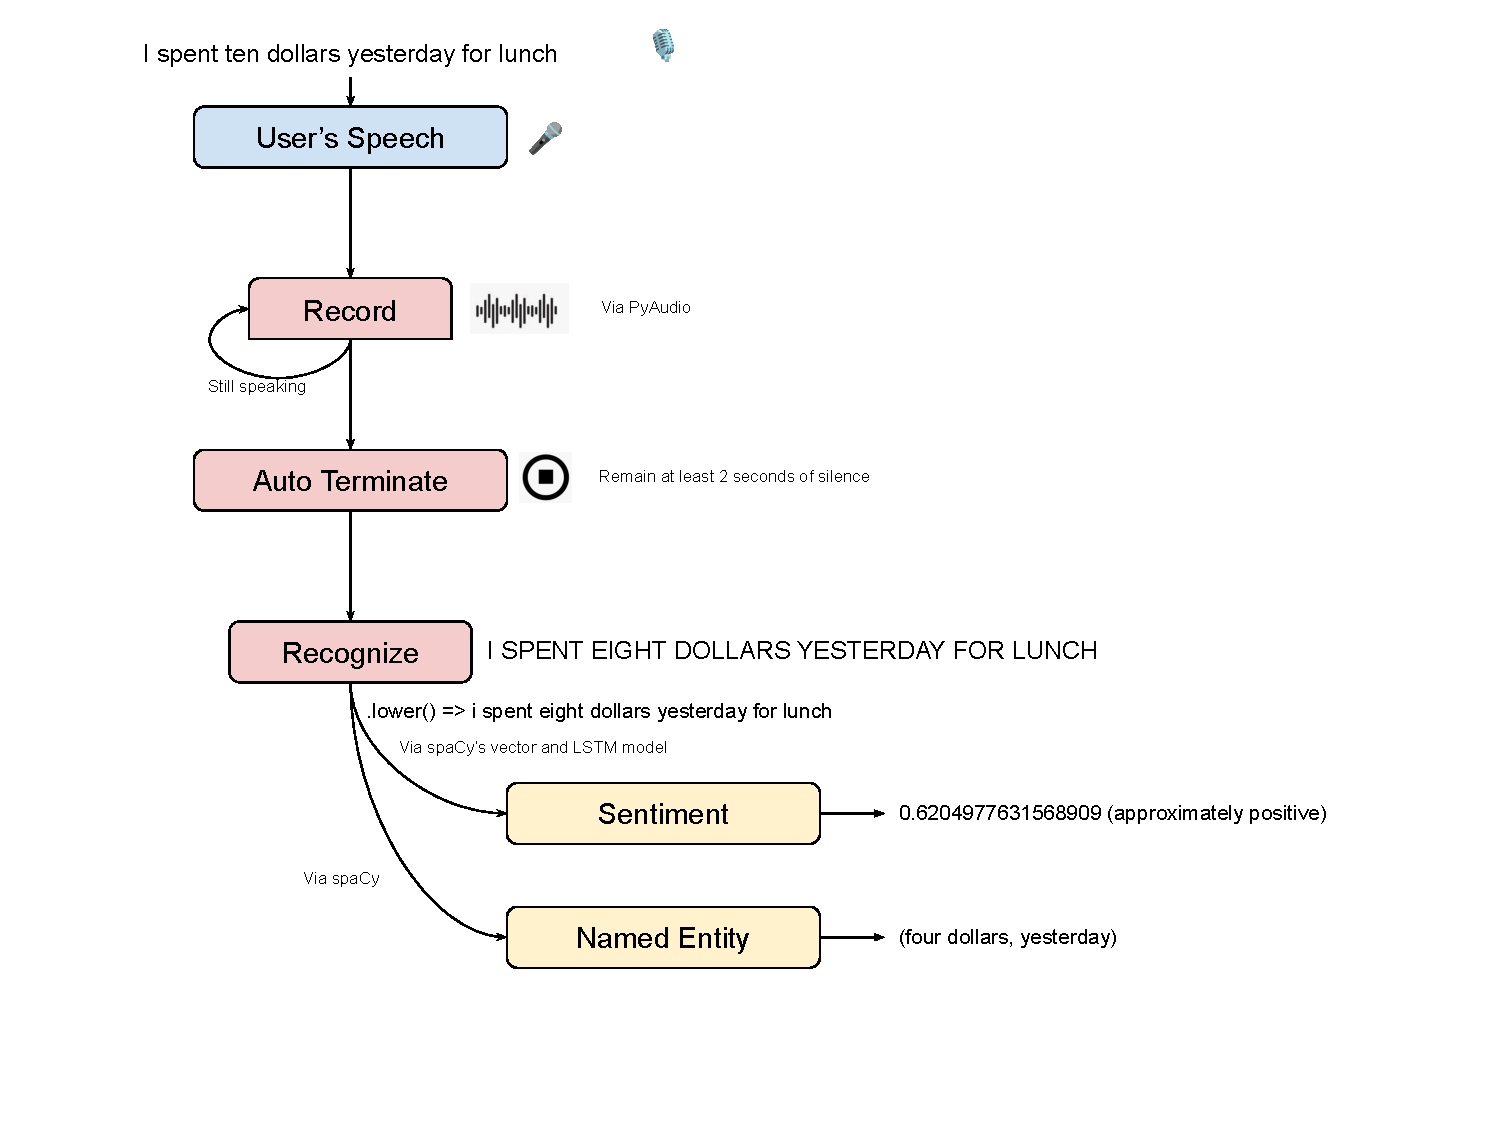
\includegraphics[width=0.8\textwidth]{./figures/audio-arch}
        \caption{The audio process system of \textbf{Aurora Echo}.}
        \label{fig:audio-process}
    \end{figure}

    The Audio Process System of \textbf{Aurora Echo} is responsible for recording the audio feedback and converting it into text.
    We also require the system to initially recognize the named entity and the sentiment of the speech.

    \subsubsection{Audio Recording}\label{subsubsec:audio-rec}

    Through \texttt{PyAudio}\cite{mark2018} library, we can record the audio feedback, and stop recording after \qty{2}{\second} of silence.

    According to the formula of calculating RMS level of the signal in \unit{\decibel} (formula \ref{eq:rms}), we can calculate the RMS level of the audio feedback.

    \begin{equation}
        \mathrm{RMS} = 20 \times \log_{10} \left( \frac{1}{N} \sum_{i=1}^{N} x_i^2 \right)\label{eq:rms}
    \end{equation}

    The algorithm of the stop recording is, when the RMS level of the audio feedback is less than \qty{30}{\decibel}, we stop recording.

    \subsubsection{Audio Recognition}\label{subsubsec:audio-recog}

    Then we use the \texttt{wav2vec} model~\cite{DBLP:journals/corr/abs-2006-11477}, we can convert the audio into text.
    According to the configuration of the pilot test environment, we selected the \texttt{wav2vec2-large-960h} model, which is a pre-trained model provided by HuggingFace and Facebook.

    The result of the audio recognition is a text with all capital letters, and we used \texttt{spaCy}\cite{spacy2,Honnibal_spaCy_Industrial-strength_Natural_2020} library to load the sentence.

    \subsubsection{Sentiment Analysis}\label{subsubsec:sentiment}

    The sentiment analysis is a logistic regression model trained on the \texttt{IMDb}\cite{zm1y-b270-20, maas-EtAl:2011:ACL-HLT2011} dataset.
    We use the LSTM\cite{43905} model to train the sentiment analysis model.

    \subsubsection{Named Entity Recognition}\label{subsubsec:ner}

    We directly use the \texttt{spaCy} library to recognize the named entity in the text.

    \subsection{Visual Recognition System}\label{subsec:visual}

    The visual recognition system involves the \texttt{MediaPipe} library to recognize the face position and the gesture, and a fine-tuned ResNet-34~\cite{DBLP:journals/corr/HeZRS15} for the facial emotion recognition.

    \begin{figure}[hhhh]
        \centering
        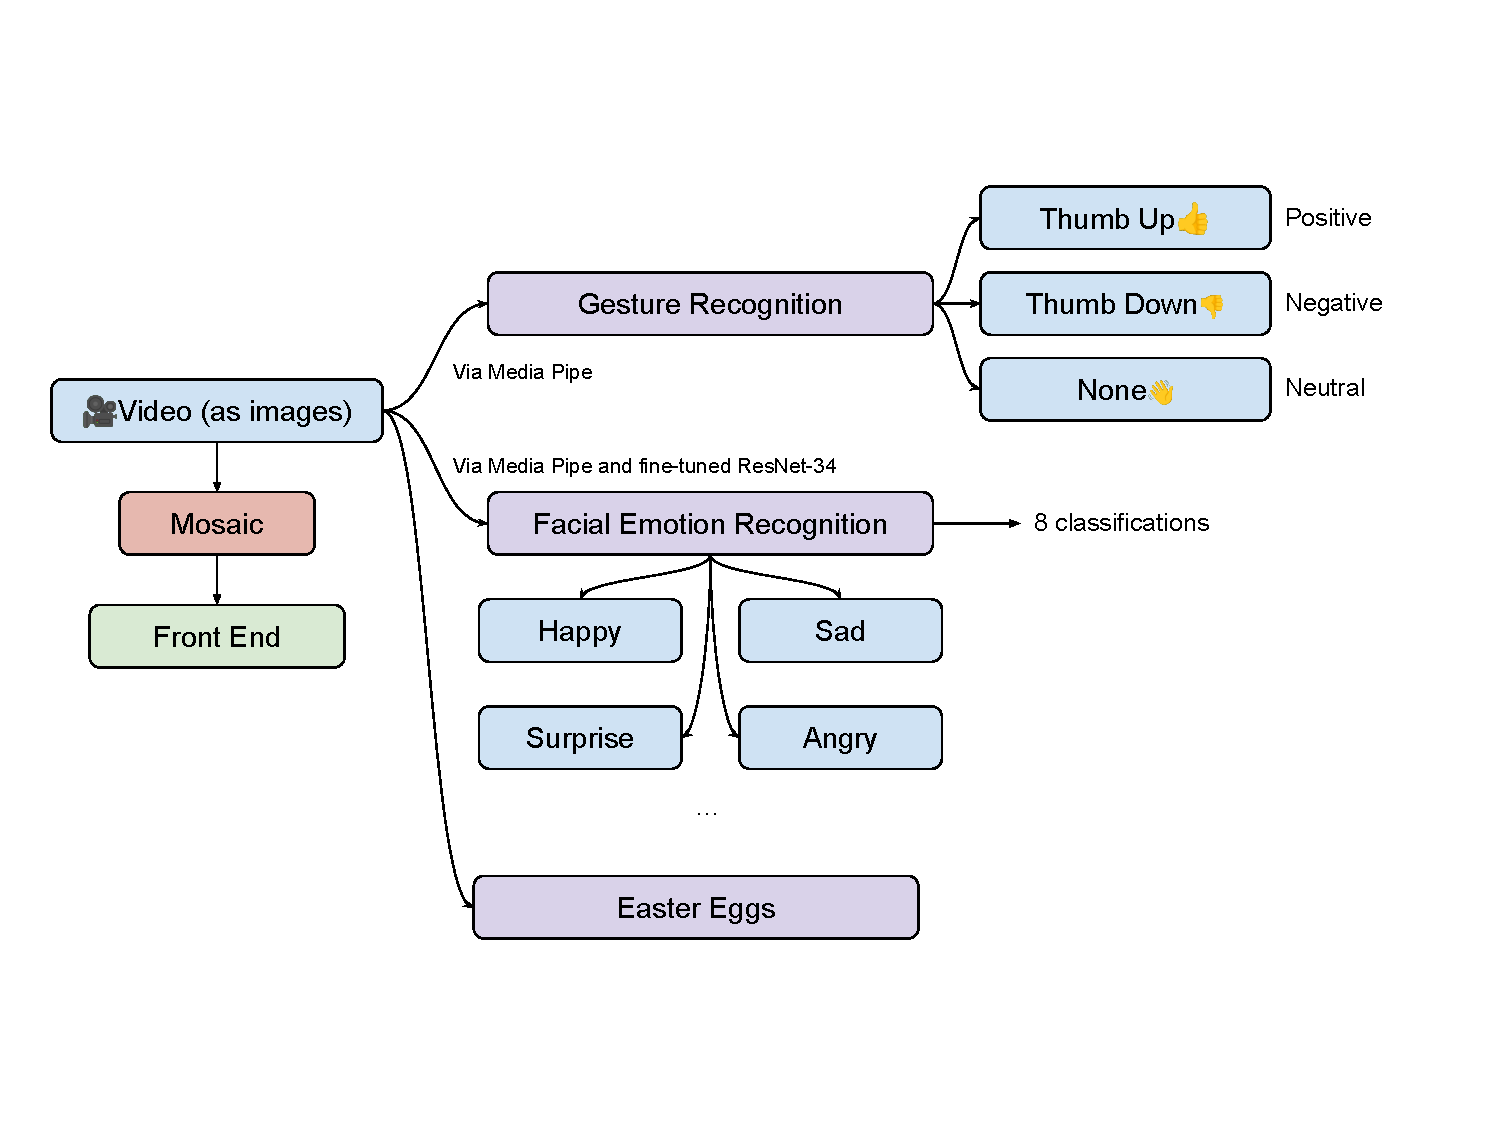
\includegraphics[width=0.8\textwidth]{./figures/vision-arch}
        \caption{The visual recognition system of \textbf{Aurora Echo}.}
        \label{fig:visual-process}
    \end{figure}

    The figure~\ref{fig:visual-process} shows the visual recognition system of \textbf{Aurora Echo}.

    \subsubsection{Facial Emotion Recognition}

    Through the \texttt{MediaPipe} library, we can recognize the face position and the facial emotion of the feedback giver.

    We normalized the image with following steps:

    \begin{enumerate}
        \item Recognize the face via \texttt{MediaPipe}.
        \item Crop the face region.
        \item Resize the face region to $256 \times 256$.
        \item Automatically adjust the brightness, contrast, and saturation, and automatically rotate and flip the image.
        \item Normalize the image.
    \end{enumerate}

    Then, we adjust the \texttt{fc} layer of the fine-tuned ResNet-34 model to recognize the facial emotion.

    The datasets are collected from \texttt{Kaggle}\cite{tapakah68_2023,kapadnis_2024}, and artificially collected them into angry, disgust, fear, happy, neutral, sad, and surprise.

    \subsubsection{Gesture Recognition}

    The gesture recognition is an accessibility function that helps the model knows the feedback giver's reaction more.
    We do not apply the ML model to the gesture recognition, but we use the \texttt{MediaPipe} library to recognize the gesture.
    Then we classified the gesture into 3 categories: thumbs up, thumbs down, and others.

    \subsection{Large Language Model Integration}\label{subsec:llm}

    The Large Language Model (LLM) is the core of the feedback analysis system.

    Considering the environment, we selected \texttt{Llama-3.1-8B}\cite{llama3modelcard,llama-3.1}\footnote[1]{Actually the model always ends with \texttt{-Instruct}, but for the sake of typography, we just ignored the suffix.}, or \texttt{Qwen2-1.5B}\cite{qwen2} as the offline LLM, or \texttt{gpt-4o-mini}\cite{gpt-4o-mini} or \texttt{Llama-3.1-405B} as the online LLM\@.

    The LLM is responsible for summarizing the feedback, analyzing the feedback, and generating the response.

    The invocation prompt is attached in the appendix.

    \section{Why Aurora Echo?}\label{sec:why}

    Using \textbf{Aurora Echo} means that you are using a vivid and direct feedback system.
    It not only pursues the directness of the feedback, a deep integration of LLMs, and a privacy-guaranteed system.

    \subsection{Security and Privacy}\label{subsec:security}

    The security issue of artificial intelligence is a hot topic.
    Calling unauthorized APIs, or storing the data without permission, is a serious problem.
    In \textbf{Aurora Echo}, system not only provides interfaces for calling the APIs, but also recommend users who have the ability to run the model locally.

    Taking \texttt{Qwen2-1.5B} as an example, the performance requirements is lower than other models, but its usability is still guaranteed for the feedback analysis.
    We tested the model on Apple's M2 Pro, we can generate the response in about \qty{3}{\minute}.
    It may be slow, but the performance of devices running Large Language Models are better.

    We also provide API to OpenAI's ChatGPT-4o Mini.
    The model is a smaller version of ChatGPT-4o, which is a model that can generate the response in real-time.

    \subsection{Multimodal Feedback}\label{subsec:multimodal}

    Not only the text feedback, but also the audio-visual feedback is provided.
    It enhances the directness of the feedback, reflecting the most immediate aspect of the feedback giver.
    Though Large Language Models now are available to directly have conversations ``face''-to-face, costs may be higher than this system.

    \section{Comparison}\label{sec:comparison}

    The ChatGPT-4o can understand the video very well, so it can also abstract the feedback from the video. \cite{tang2024videounderstandinglargelanguage}
    But why we do not use ChatGPT-4o to abstract the feedback from the video?

    \subsection{Cost}\label{subsec:cost}

    Just taking the image module as an example, and the audio module similar.

    According to a small calculation, if you put a \qty{30}{\second} video to a LLM, you may spend about \qty{200}{GiB} of data, and about \qty{8}{\kilo\watt} energy for parsing the video. \cite{husom2024pricepromptingprofilingenergy, samsi2023wordswattsbenchmarkingenergy}

    If using the Aurora Echo, you can just run the model on the local CPU, even on the web (with WASM and MediaPipe web), you can save a lot of energy and data.

    Suppose there were a video in \qty{30}{\second} (30 fps).
    We just need to recognize 900 frames of the gesture and face.
    Amount parameters of models (including the facial emotion recognition) related to image processing is at most 2 Billion parameters.

    Also, the extraction of LLM is also energy-consuming.

    Though finally Aurora Echo uses the LLM to generate the \texttt{function call} and to summarize, this kind of task doesn't require a lot of parameters, and the model can also run on the local CPU\@.

    \subsection{Privacy}\label{subsec:privacy}

    Aurora Echo runs model on the local.
    In the best case scenario, ALL the models, including the LLM, can run on local (with the help of uniformed memory from Apple Silicon, or using OpenVINO for Intel CPU).
    Through functions above, we can easily run \texttt{Qwen2-1.5B}, or \texttt{Llama-3.1-8B} on the local, once you have at lease \qty{16}{GiB} of memory.

    Also, the face is mosaic-permitted, and the video is not stored.
    What the system stores is only the report and the function-call to the database.

    \subsection{Directness}\label{subsec:directness}

    The directness of the feedback is the most important aspect of the system.

    Through Aurora Echo, we can also promptly expand the conversation with the help of LLM\@.
    We can use prompt to invoke the LLM, and have a chat to response the most immediate aspect of the feedback giver.

    \section{Conclusion}\label{sec:conclusion}

    The \textbf{Aurora Echo} system is a new feedback system that provides audio-visual feedback for the resource provider.
    Through its 3 parts, the audio process system, the visual recognition system, and the feedback analysis system, we can provide a more vivid and direct feedback system for the resource provider.
    The system is also privacy-friendly, and we provide a web interface for the resource provider to check the feedback and the analysis.

    The code of the system is available at \url{https://github.com/zzteam-rccup/aurora-echo.git}.

    The next step for the project are:

    \begin{itemize}
        \item Improve the frontend interface.
        \item Migrate the MediaPipe and the OpenCV part to the web, with the help of WASM and Rust.
        \item Add some extensions for the system.
        \item Improve the accuracy of facial emotion recognition.
        \item Optimize the performance of the system.
    \end{itemize}

    \paragraph{Acknowledgements}

    We are grateful to Shanghai Jiao Tong University for providing the summer camp, and the teachers for guidance of artificial intelligence.

    \nocite{*}
    \bibliography{./citations}
    \bibliographystyle{plain}
\end{document}
